\documentclass{article}
\usepackage{epsfig}
\usepackage{graphicx}
\usepackage[top=0.50in, bottom=0.50in, left=0.65in, right=0.75in]{geometry}
%\usepackage[a4paper, total={6in, 10in}]{geometry}
\usepackage[table]{xcolor}
\usepackage{tikz}
\usepackage{algorithm}
\usepackage{mathtools}
\usepackage{amsmath,amssymb}
\usepackage[]{algpseudocode}
\usepackage{enumitem}
\title{CS345 Theoretical Assignment 4 \\ }
\author{\vspace{2mm} \large Ayush Agarwal, 13180 \\ M.Arunothia, 13378}
\date{}
\begin{document}
\maketitle
\tableofcontents
\newpage
\section{Any Guarantee of our First-Attempt Algorithm}
\subsection{Counter Example}
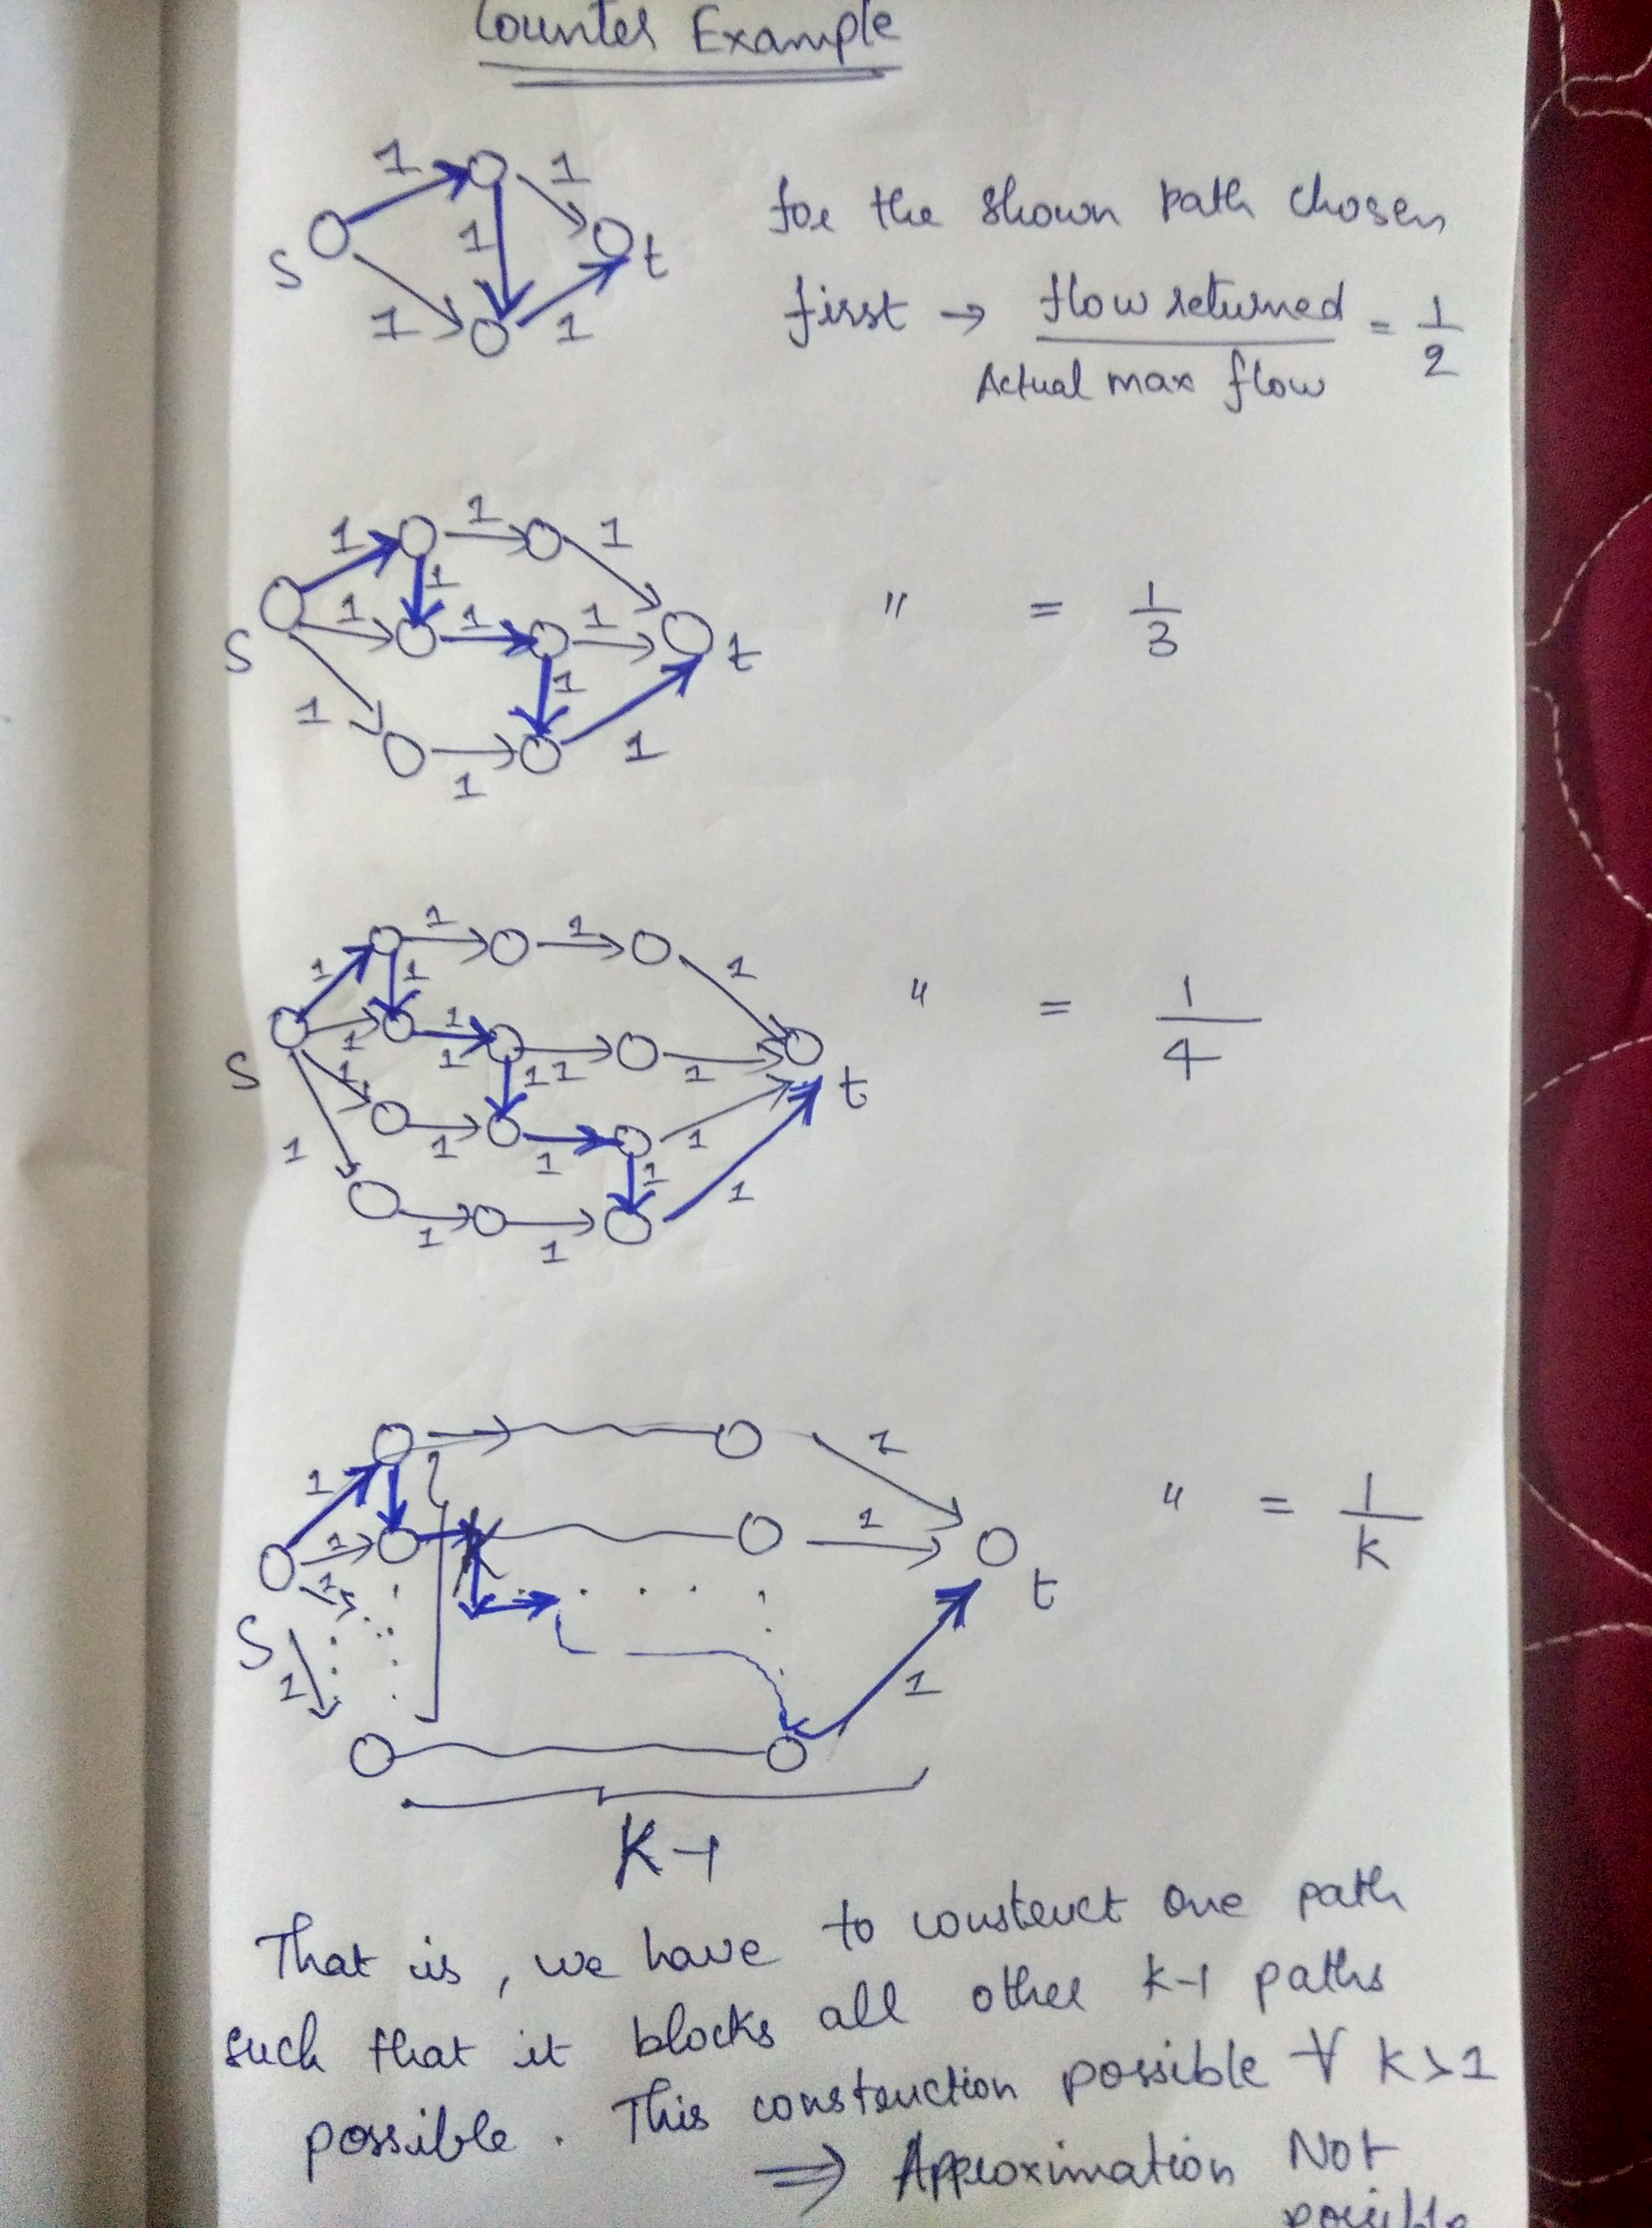
\includegraphics[scale=0.5]{1.jpg}
\newpage
\section{A max flow application}
\subsection{Without Extra Constraint}
\subsubsection{Overview}
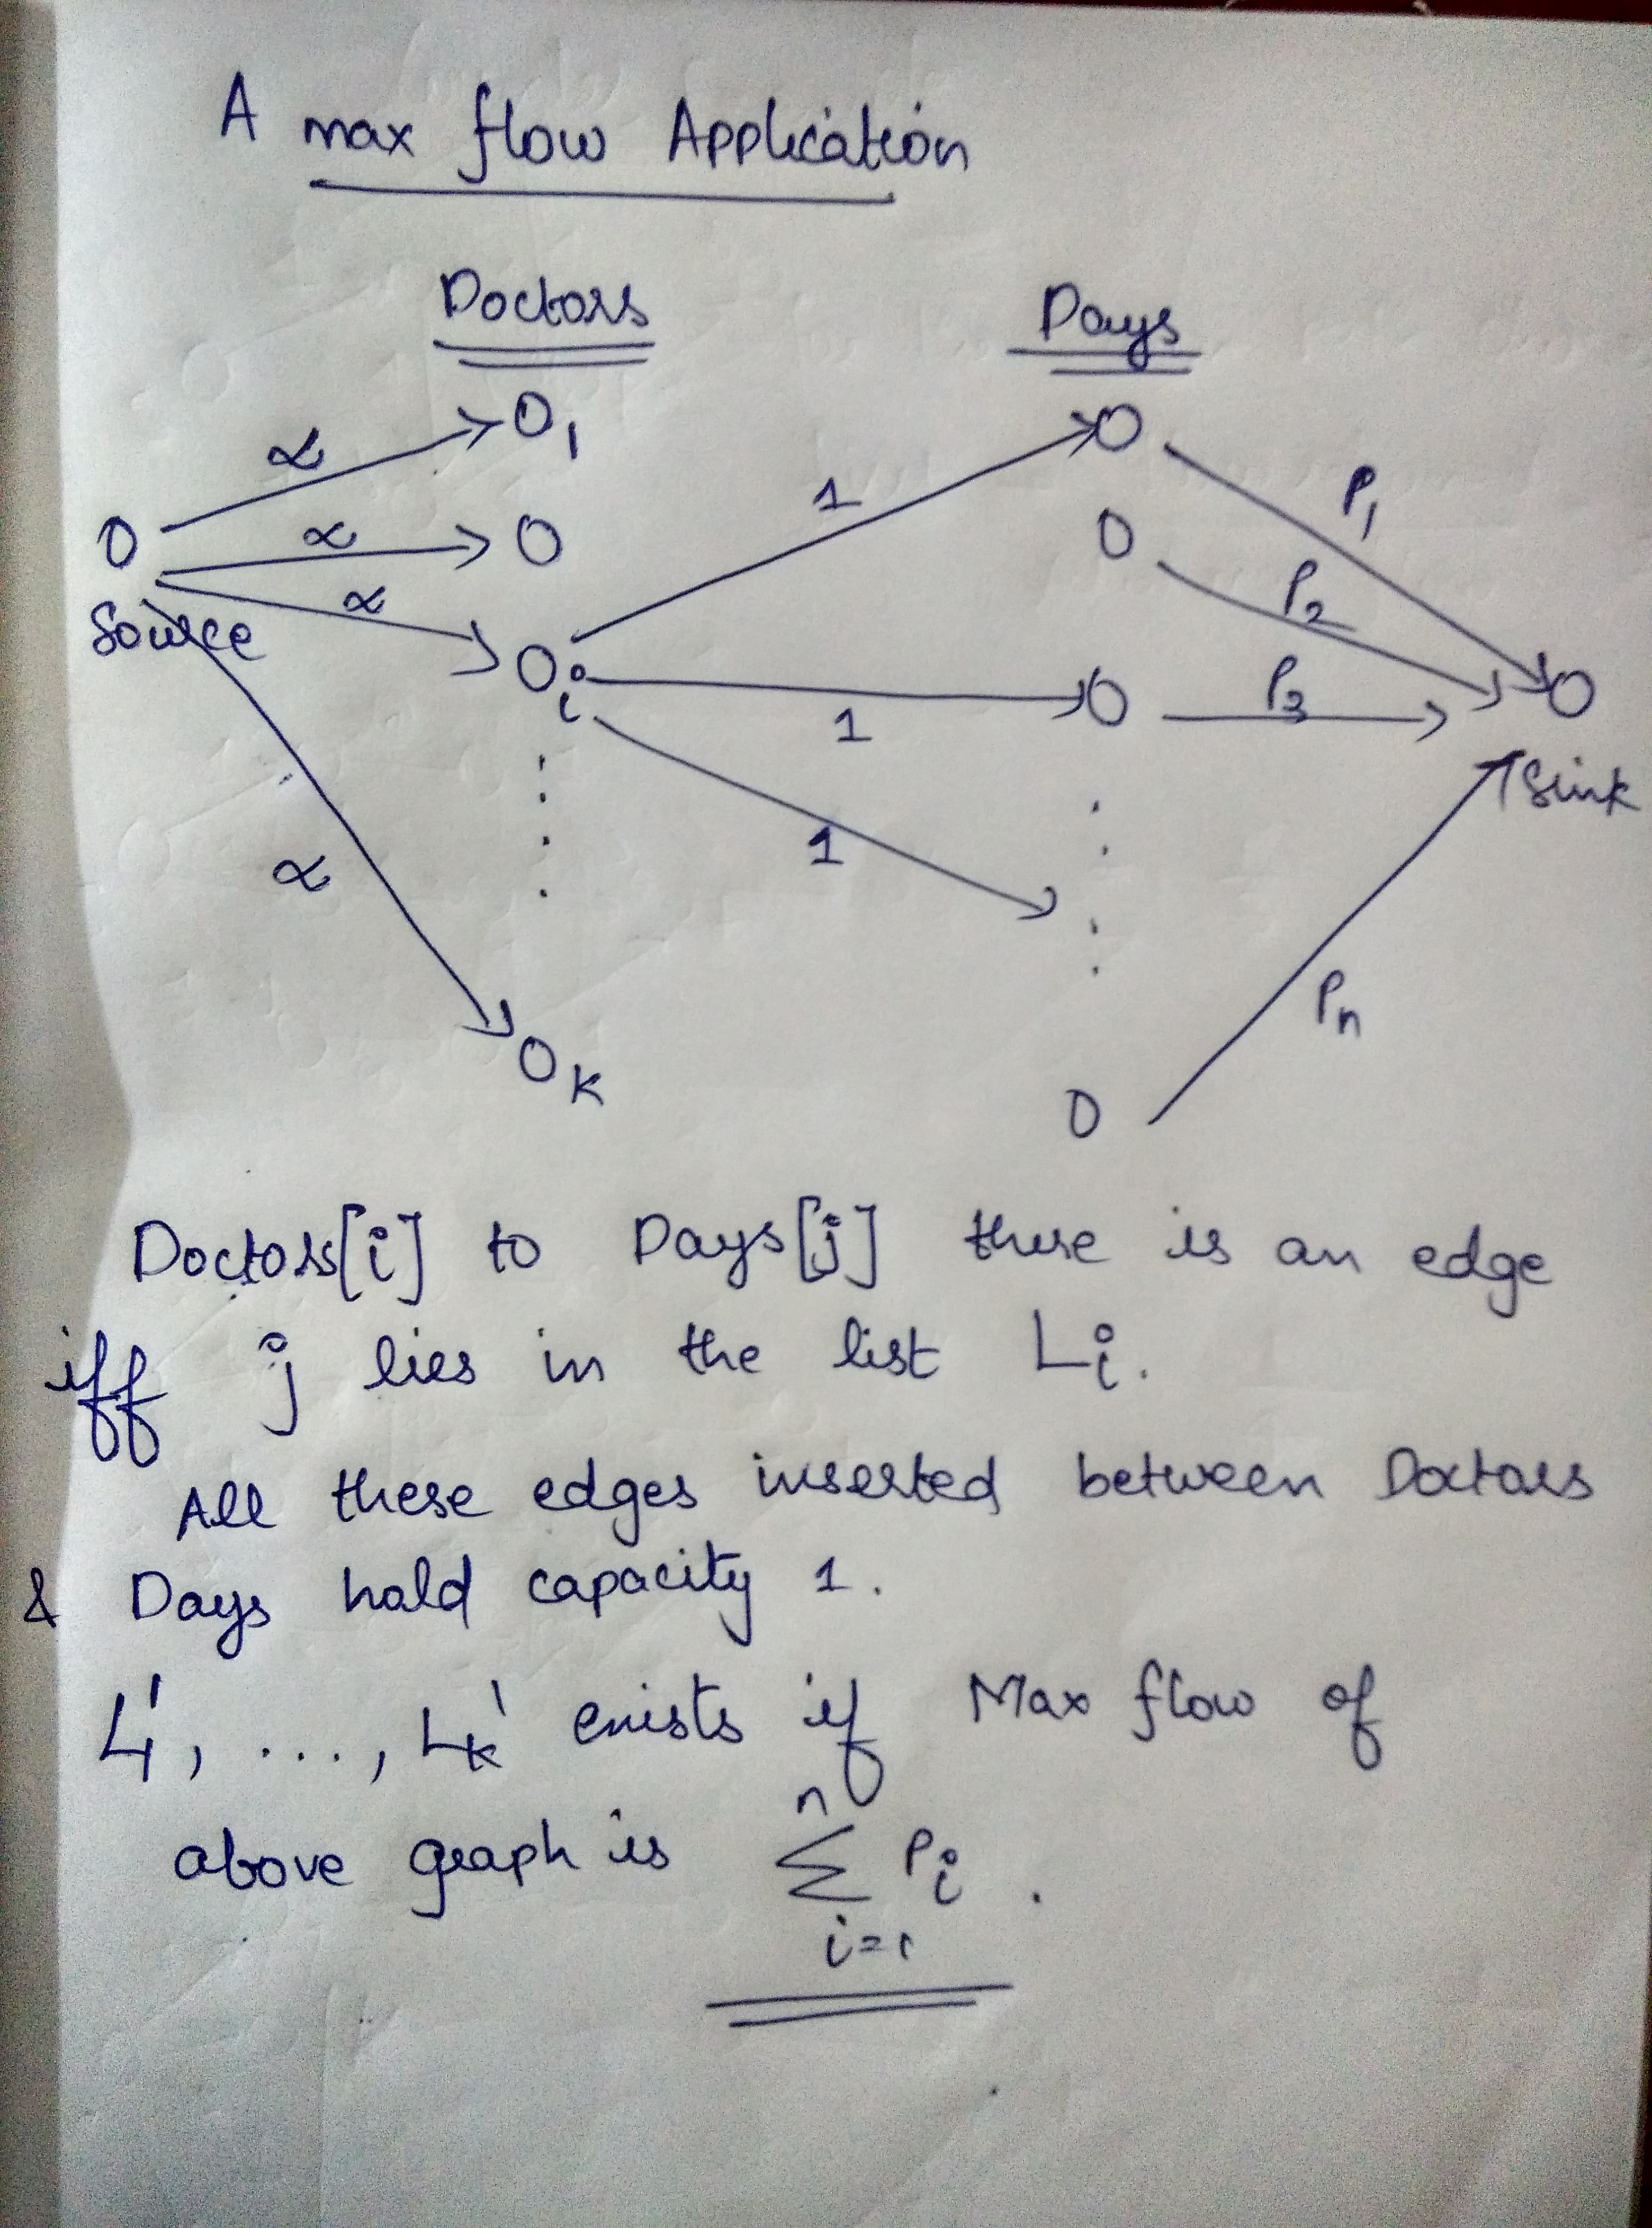
\includegraphics[scale=0.15]{3a.jpg}
\subsubsection{Notations}
$p_i$ denotes the exact number of doctors required on day $i$ \\
$L_i$ denotes the list of days where doctor $i$ is available \\
$L'_i$ denotes the list of days that doctor $i$ has to work to produce the required match. Note, $L'_i \subseteq L_i$\\
$D = \sum_{i=1}^{n} p_i$ \\
$n$ = Number of days in total \\
$k$ = Number of Doctors in total \\ 
\subsubsection{Claim}
Construction of $L'_i$s is possible if and only if the max-flow in the source-sink graph constructed (in image) is D.
\subsubsection{Proof - Part 1}
{\bf Given $L'_i$s list for all doctors, show that the max flow of source-sink graph shown above is D \\}
Construct a flow $f$ of the source-sink graph as follows. \\
$f(source,Doctor[i])$ is $|L'_i|$ - satisfies capacity constraint as these edges had infinite capacity \\
$f(Doctor[i], Day[j])$ is $1$ if $j$ lies in $L'_i$, otherwise is $0$ - satisfies capacity constraint \\
$f(Day[j],sink)$ is $p_j$ - satisfies capacity constraint \\
Flow Conservation is ensured as it is given to us that $L'_i$s of such definitions exist. \\
Hence, the above is a valid flow. \\
As the $cut-capacity$ between $sink$ and the rest of the graph is $D$, by $min-cut - max-flow$ theorem, $f$ should be a max flow of the source-sink graph. Hence, proved. 
\subsubsection{Proof - Part 2}
{\bf Given the max flow of source-sink graph to be D, show that $L'_i$s list for all doctors exist \\}
Let $f$ be the integral max-flow of the source-sink graph. (Note: Integral flow exists was proved in class) \\
Construct $L'_i$ as follows. \\
If $f(Doctor[i], Day[j])$ is $1$ then add $j$ to $L'_i$ otherwise do nothing. \\
Note: $f(Doctor[i], Day[j])$ can be only $0$ or $1$ by integral flow property. \\
The $L'_i$s thus constructed are valid as $value(f) = D$ implying every day $j$ has got the exact number of doctors wanted ($p_j$). Moreover, $L'_i \subseteq L_i$ is ensured from the construction of the source-sink graph itself. Hence, proved.
\newpage
\subsection{With Extra Constraint}
\subsubsection{Overview}
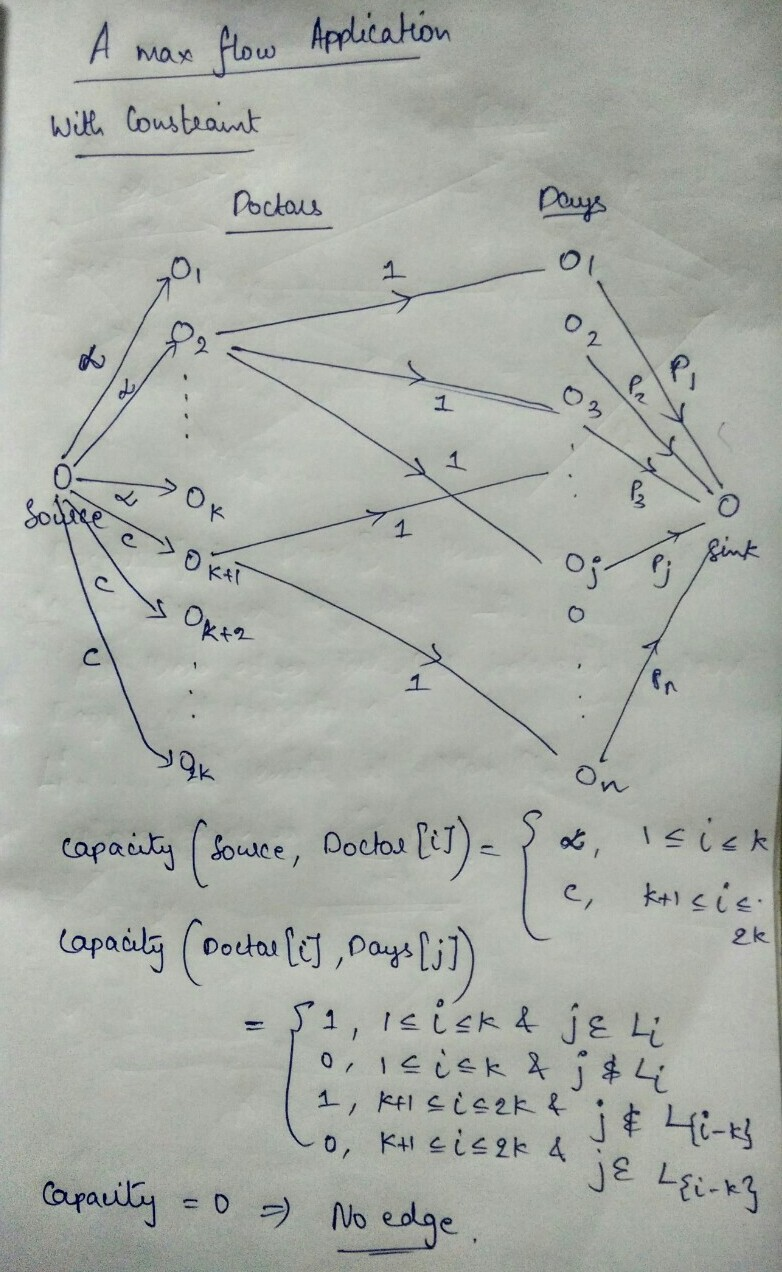
\includegraphics[scale=0.5]{3b.jpg}
\newpage
\subsubsection{Notations}
$p_i$ denotes the exact number of doctors required on day $i$ \\
$L_i$ denotes the list of days where doctor $i$ is available \\
$L'_i$ denotes the list of days that doctor $i$ has to work to produce the required match. \\
$K_i = L_i \cap  L'_i$ \\
$C_i = L'_i - K_i$ \\ 
$D = \sum_{i=1}^{n} p_i$ \\
$n$ = Number of days in total \\
$k$ = Number of Doctors in total \\ 
\subsubsection{Claim}
Construction of $L'_i$s is possible if and only if the max-flow in the source-sink graph constructed (in image) is D.
\subsubsection{Proof - Part 1}
{\bf Given $L'_i$s list for all doctors, show that the max flow of source-sink graph shown above is D \\}
Construct a flow $f$ of the source-sink graph as follows. \\
If $i \leq k$ then \\
$f(source,Doctor[i])$ is $|K_i|$ - satisfies capacity constraint as these edges had infinite capacity \\
$f(Doctor[i], Day[j])$ is $1$ if $j$ lies in $K_i$, otherwise is $0$ - satisfies capacity constraint \\
If $i > k$ then \\
$f(source,Doctor[i])$ is $|C_i|$ - satisfies capacity constraint by definition of $L'_i$s existence. \\
$f(Doctor[i], Day[j])$ is $1$ if $j$ lies in $C_i$, otherwise is $0$ - satisfies capacity constraint \\
 \\
$f(Day[j],sink)$ is $p_j$ - satisfies capacity constraint \\
 \\
Flow Conservation is ensured as it is given to us that $L'_i$s of such definitions exist. \\
Hence, the above is a valid flow. \\
As the $cut-capacity$ between $sink$ and the rest of the graph is $D$, by $min-cut - max-flow$ theorem, $f$ should be a max flow of the source-sink graph. Hence, proved. 
\subsubsection{Proof - Part 2}
{\bf Given the max flow of source-sink graph to be D, show that $L'_i$s list for all doctors exist \\}
Let $f$ be the integral max-flow of the source-sink graph. (Note: Integral flow exists was proved in class) \\
Construct $L'_i$ as follows. \\
If $f(Doctor[i], Day[j])$ or $f(Doctor[i+k], Day[j])$ is $1$ then add $j$ to $L'_i$ otherwise do nothing. \\
Note: $f(Doctor[i], Day[j])$ can be only $0$ or $1$ by integral flow property. \\
The $L'_i$s thus constructed are valid as $value(f) = D$ implying every day $j$ has got the exact number of doctors wanted ($p_j$). Moreover, both $f(Doctor[i], Day[j])$ and $f(Doctor[i+k], Day[j])$ will not be together $1$ from the construction of source-sink graph itself. Hence, proved.
\end{document}